\documentclass[a4paper]{article}
\usepackage[svgnames]{xcolor}
\usepackage{amsmath,amsfonts,amssymb}
\usepackage{geometry}
\usepackage{fancyhdr}
\usepackage{graphicx}
\usepackage{titlesec}
\usepackage{caption}
\usepackage{subcaption}
\usepackage{tikz}
\usepackage{tcolorbox}
\usepackage{float} % For figure positioning
\usepackage{lipsum}
\usepackage{mdframed}
\usepackage{amsmath}
\usepackage{amsmath,amsfonts,amssymb}
\usepackage{graphicx}
\usepackage{enumitem}
\usepackage{titlesec}
\usepackage{fancyhdr}
\usepackage{hyperref}
% \usepackage{floatrow}
\usepackage{listings}
\usepackage{geometry}
\usepackage{fancyhdr}
\usepackage{empheq}
\usepackage[svgnames]{xcolor}
\usepackage{xpatch}


\geometry{margin=0.5in}
\pagestyle{fancy}
\fancyhf{}

% Header and Footer
% \fancyhead[L]{\includegraphics[width=1.5cm]{logo.png}} % Add your logo
\fancyhead[C]{\textbf{\color{blue!70}CS663 Assignment-3}}
% \fancyhead[R]{\color{blue!70}Saksham Rathi}
\fancyfoot[C]{\thepage}

% Custom Section Color and Format
\titleformat{\section}
{\color{purple!80!black}\normalfont\Large\bfseries}
{\thesection}{1em}{}

% Beautiful Title with TikZ
\newcommand{\cooltitle}[1]{%
  \begin{tikzpicture}
    \node[fill=blue!20,rounded corners=10pt,inner sep=10pt] (box)
    {\Huge \bfseries \color{black} #1};
  \end{tikzpicture}
}

% Stylish Solution Environment with float option enabled
% Stylish Solution Environment with breakable option
% Stylish Solution Environment with mdframed
\newenvironment{solution}[2][]{%
    \begin{mdframed}[linecolor=green!60!black, linewidth=2pt, roundcorner=10pt, backgroundcolor=green!5!white, skipabove=12pt, skipbelow=12pt]%
        \textbf{\large #2} % Heading in bold and large font
        \par\noindent\rule{\textwidth}{0.4pt} % Horizontal line after heading
        \vspace{0.5em} % Small vertical space
}{%
    \end{mdframed}%
}





\title{\cooltitle{CS663 Assignment-3}}
\author{{\bf Saksham Rathi, Kavya Gupta, Shravan Srinivasa Raghavan} \\
\small Department of Computer Science, \\
Indian Institute of Technology Bombay \\}
\date{}

\begin{document}

\maketitle
\section*{Question 3}

\begin{solution}{Solution}
    Here are the original and the noisy versions of the images:
\begin{figure}[H]
    \centering
    % First subfigure
    \begin{subfigure}[b]{0.3\textwidth}
        \centering
        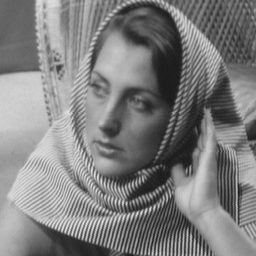
\includegraphics[width=\textwidth]{../images/barbara256.png}
        \caption{Original}
        \label{fig:subfig1}
    \end{subfigure}
    % Second subfigure
    \begin{subfigure}[b]{0.3\textwidth}
        \centering
        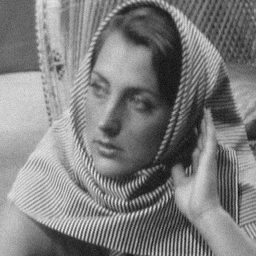
\includegraphics[width=\textwidth]{../images/noisy_barbara256.png}
        \caption{Noisy }
        \label{fig:subfig2}
    \end{subfigure}
    \caption{Versions of barbara image}
    \label{fig:overall}
\end{figure}

\begin{figure}[H]
    \centering
    % First subfigure
    \begin{subfigure}[b]{0.3\textwidth}
        \centering
        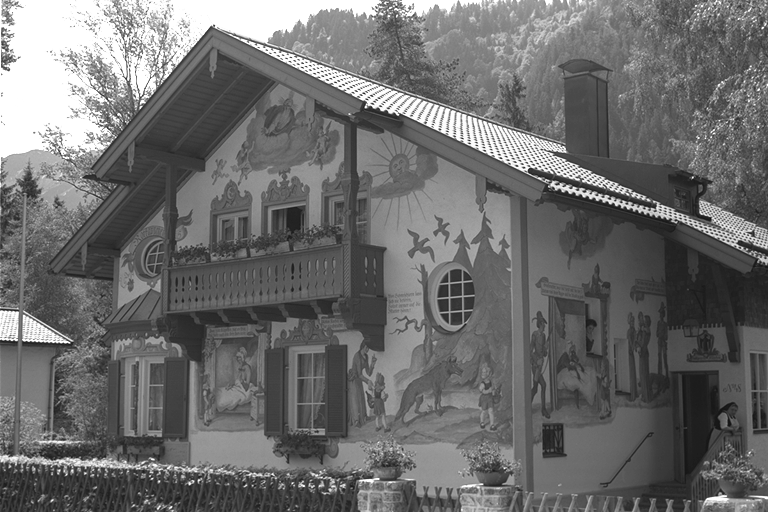
\includegraphics[width=\textwidth]{../images/kodak24.png}
        \caption{Original}
        \label{fig:subfig1}
    \end{subfigure}
    % Second subfigure
    \begin{subfigure}[b]{0.3\textwidth}
        \centering
        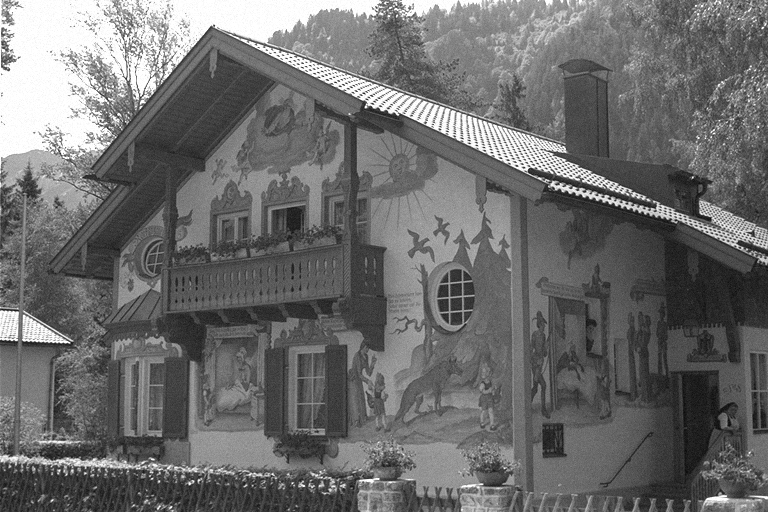
\includegraphics[width=\textwidth]{../images/noisy_kodak24.png}
        \caption{Noisy }
        \label{fig:subfig2}
    \end{subfigure}
    \caption{Versions of kodak image}
    \label{fig:kodak}
\end{figure}

The code for this question is present in {../code/myMainScript.m}, \\ {../code/mybilateralfilter.m} and {../code/mymeanshiftfilter.m}. The window size of the bilateral filter and the meanshift filter is chosen to be $2\times [3*\sigma_s] + 1$, where $[]$ denotes the ceiling function.


Here are the results of applying bilateral filter on noisy ($\sigma = 5$) barbara image with various values of $\sigma_s$ and $\sigma_r$:

\begin{figure}[H]
    \centering
    % First subfigure
    \begin{subfigure}[b]{0.24\textwidth}
        \centering
        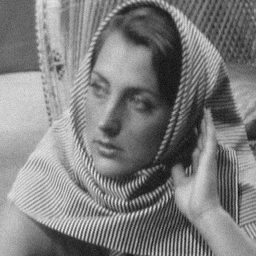
\includegraphics[width=\textwidth]{../images/noisy_barbara256.png}
        \caption{sigma=5}
        \label{Noisy }
    \end{subfigure}
    % Second subfigure
    \begin{subfigure}[b]{0.24\textwidth}
        \centering
        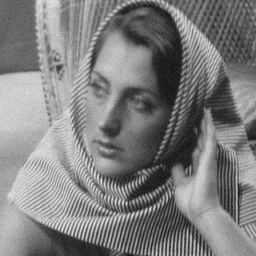
\includegraphics[width=\textwidth]{../images/filtered_barbara256_bilateral_sigma_s_2_sigma_r_2.png}
        \caption{$\sigma_s=2;\sigma_r=2$}
        \label{fig:subfig2}
    \end{subfigure}
    % Third subfigure
    \begin{subfigure}[b]{0.24\textwidth}
        \centering
        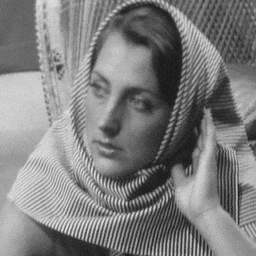
\includegraphics[width=\textwidth]{../images/filtered_barbara256_bilateral_sigma_s_3_sigma_r_15.png}
        \caption{$\sigma_s=3;\sigma_r=15$}
        \label{fig:subfig3}
    \end{subfigure}
    \begin{subfigure}[b]{0.24\textwidth}
        \centering
        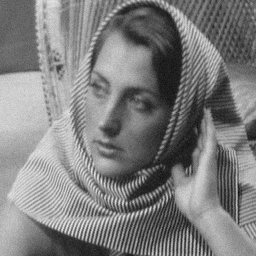
\includegraphics[width=\textwidth]{../images/filtered_barbara256_bilateral_sigma_s_15_sigma_r_3.png}
        \caption{$\sigma_s=15;\sigma_r=3$}
        \label{fig:subfig3}
    \end{subfigure}
    
    \caption{Bilateral Versions of barbara image }
    \label{fig:overall}
\end{figure}

If we talk with respect to the face of the barbara image, we can see that the image with $\sigma_s = 3$ and $\sigma_r = 15$ has a more clear face. Higher $\sigma_s$ actually incorporates intensity values from far neighbourhood too, which decreases the clarity of the face. Higher $\sigma_r$ means that the intensity values are taken from a larger range of intensity values, which makes the face more clear. Edges are preserved for all the images. All the other parts of the image have similar texture and hence the difference is not very visible.


Here are the results of applying mean-shift filter on noisy ($\sigma = 5$) barbara image with various values of $\sigma_s$ and $\sigma_r$:

\begin{figure}[H]
    \centering
    % First subfigure
    \begin{subfigure}[b]{0.24\textwidth}
        \centering
        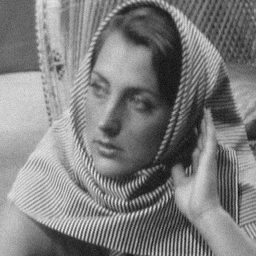
\includegraphics[width=\textwidth]{../images/noisy_barbara256.png}
        \caption{sigma=5}
        \label{Noisy }
    \end{subfigure}
    % Second subfigure
    \begin{subfigure}[b]{0.24\textwidth}
        \centering
        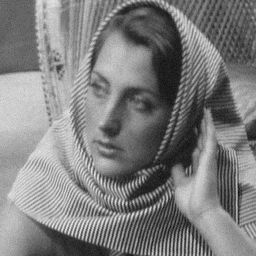
\includegraphics[width=\textwidth]{../images/filtered_barbara256_meanshift_sigma_s_2_sigma_r_2.png}
        \caption{$\sigma_s=2;\sigma_r=2$}
        \label{fig:subfig2}
    \end{subfigure}
    % Third subfigure
    \begin{subfigure}[b]{0.24\textwidth}
        \centering
        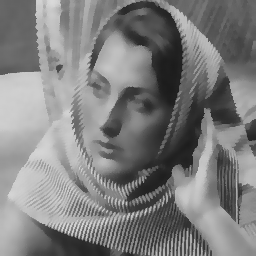
\includegraphics[width=\textwidth]{../images/filtered_barbara256_meanshift_sigma_s_3_sigma_r_15.png}
        \caption{$\sigma_s=3;\sigma_r=15$}
        \label{fig:subfig3}
    \end{subfigure}
    \begin{subfigure}[b]{0.24\textwidth}
        \centering
        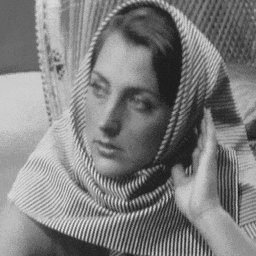
\includegraphics[width=\textwidth]{../images/filtered_barbara256_meanshift_sigma_s_15_sigma_r_3.png}
        \caption{$\sigma_s=15;\sigma_r=3$}
        \label{fig:subfig3}
    \end{subfigure}
    
    \caption{Mean-shift Versions of kodak image }
    \label{fig:overall}
\end{figure}

If we talk with respect to the face of the barbara image, we can see that the image with $\sigma_s=3$ and $\sigma_r=15$ has a blurred face. This is because a high value of $\sigma_r$ incorporates values from a larger intensity range which is clearly not good in this case. Moreover for this case, the edges are not preserved too. The image with $\sigma_s=15$ and $\sigma_r=3$ has more clarity over the image with $\sigma_s=2$ and $\sigma_r=2$. Edges are preserved for both of the images. Moreover, the texture of all the other parts of the image is more clear for both of these than the third one.


Here are the results of applying bilateral filter on noisy ($\sigma = 5$) kodak image with various values of $\sigma_s$ and $\sigma_r$:

\begin{figure}[H]
    \centering
    % First subfigure
    \begin{subfigure}[b]{0.24\textwidth}
        \centering
        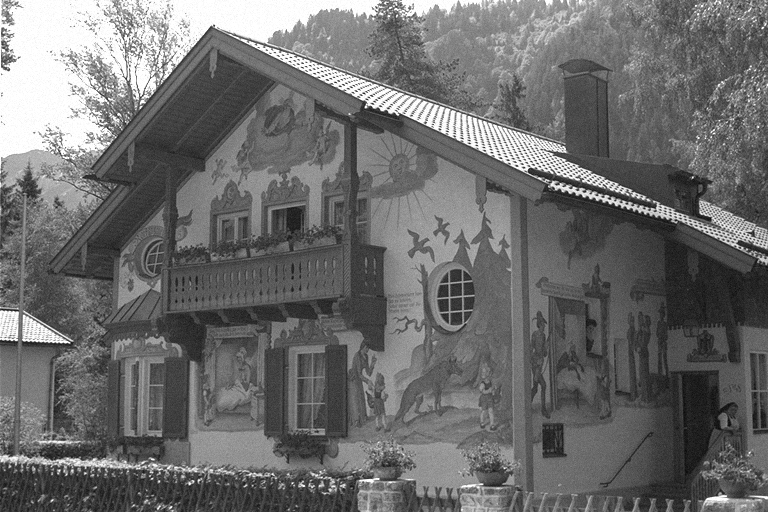
\includegraphics[width=\textwidth]{../images/noisy_kodak24.png}
        \caption{sigma=5}
        \label{Noisy }
    \end{subfigure}
    % Second subfigure
    \begin{subfigure}[b]{0.24\textwidth}
        \centering
        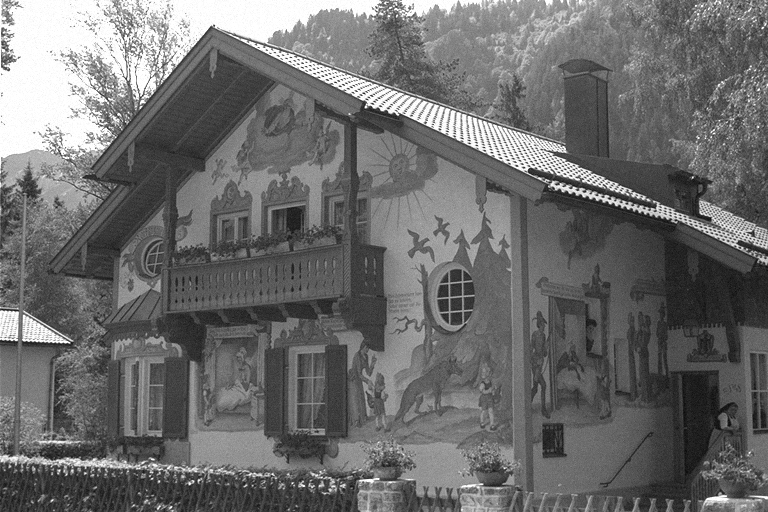
\includegraphics[width=\textwidth]{../images/filtered_kodak24_bilateral_sigma_s_2_sigma_r_2.png}
        \caption{$\sigma_s=2;\sigma_r=2$}
        \label{fig:subfig2}
    \end{subfigure}
    % Third subfigure
    \begin{subfigure}[b]{0.24\textwidth}
        \centering
        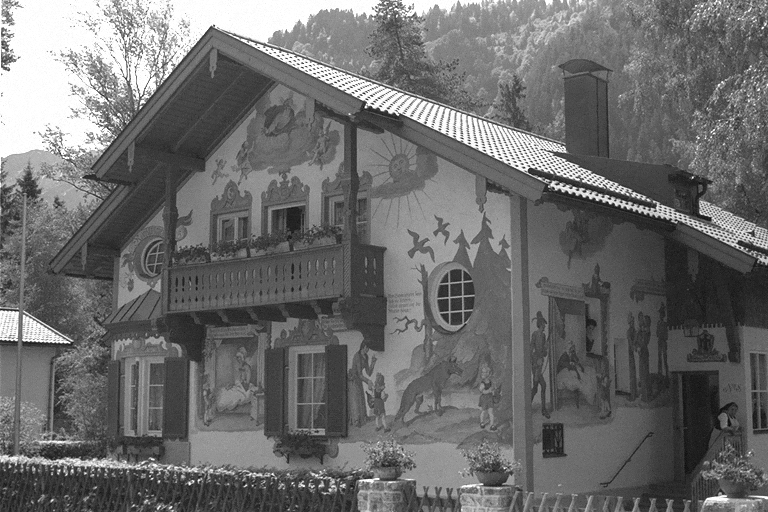
\includegraphics[width=\textwidth]{../images/filtered_kodak24_bilateral_sigma_s_3_sigma_r_15.png}
        \caption{$\sigma_s=3;\sigma_r=15$}
        \label{fig:subfig3}
    \end{subfigure}
    \begin{subfigure}[b]{0.24\textwidth}
        \centering
        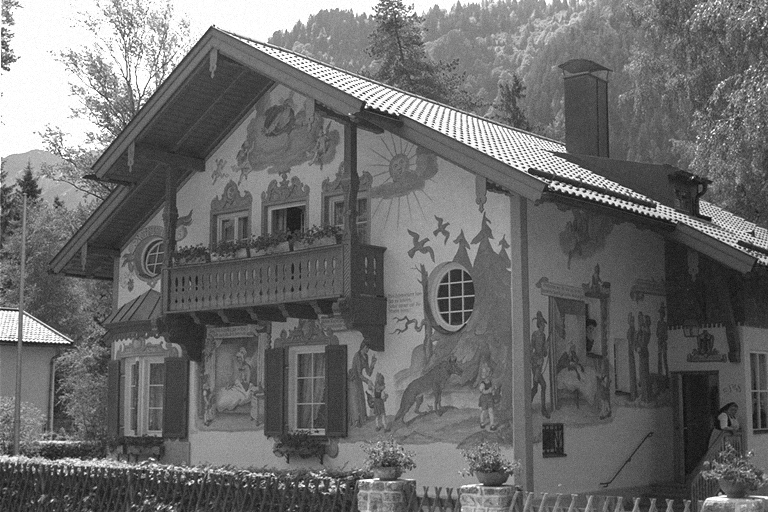
\includegraphics[width=\textwidth]{../images/filtered_kodak24_bilateral_sigma_s_15_sigma_r_3.png}
        \caption{$\sigma_s=15;\sigma_r=3$}
        \label{fig:subfig3}
    \end{subfigure}
    
    \caption{Bilateral Versions of kodak image }
    \label{fig:overall}
\end{figure}


Overall, the quality of the image with $\sigma_s=2$ and $\sigma_r=2$ is the best. One of the possible reasons for this is that kodak24 has a variety of intensities and edges. A high value of $\sigma_s$ incorporates values from a larger neighbourhood which is not good in this case. A high value of $\sigma_r$ incorporates values from a larger intensity range which is also not good in this case. The image with $\sigma_s=3$ and $\sigma_r=15$ has more clarity over the image with $\sigma_s=15$ and $\sigma_r=3$. Edges are preserved for all the images. The overall texture looks quite similar for all the three images. 

Here are the results of applying mean-shift filter on noisy ($\sigma = 5$) kodak image with various values of $\sigma_s$ and $\sigma_r$:

\begin{figure}[H]
    \centering
    % First subfigure
    \begin{subfigure}[b]{0.24\textwidth}
        \centering
        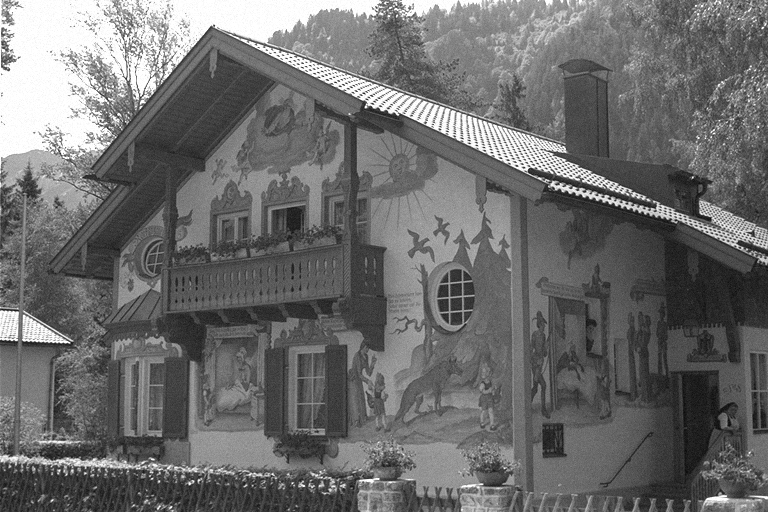
\includegraphics[width=\textwidth]{../images/noisy_kodak24.png}
        \caption{sigma=5}
        \label{Noisy }
    \end{subfigure}
    % Second subfigure
    \begin{subfigure}[b]{0.24\textwidth}
        \centering
        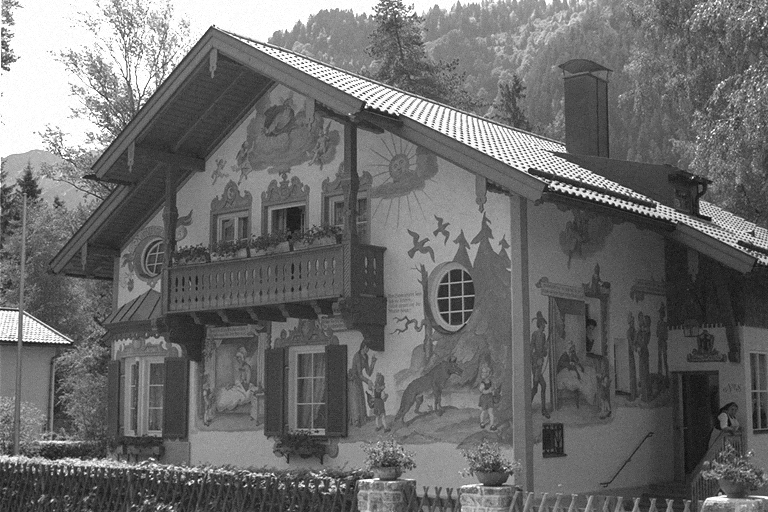
\includegraphics[width=\textwidth]{../images/filtered_kodak24_meanshift_sigma_s_2_sigma_r_2.png}
        \caption{$\sigma_s=2;\sigma_r=2$}
        \label{fig:subfig2}
    \end{subfigure}
    % Third subfigure
    \begin{subfigure}[b]{0.24\textwidth}
        \centering
        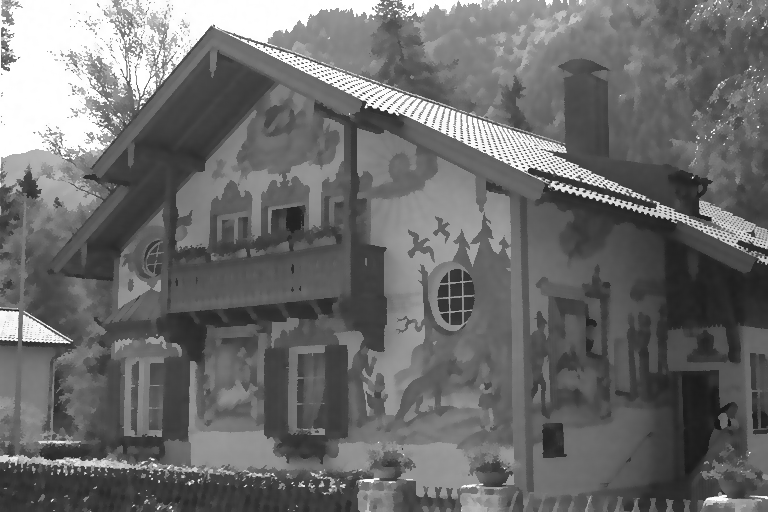
\includegraphics[width=\textwidth]{../images/filtered_kodak24_meanshift_sigma_s_3_sigma_r_15.png}
        \caption{$\sigma_s=3;\sigma_r=15$}
        \label{fig:subfig3}
    \end{subfigure}
    \begin{subfigure}[b]{0.24\textwidth}
        \centering
        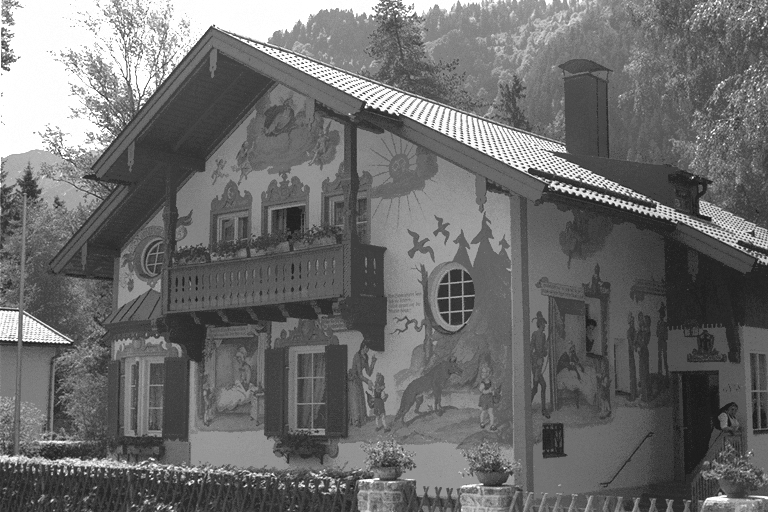
\includegraphics[width=\textwidth]{../images/filtered_kodak24_meanshift_sigma_s_15_sigma_r_3.png}
        \caption{$\sigma_s=15;\sigma_r=3$}
        \label{fig:subfig3}
    \end{subfigure}
    
    \caption{Mean-shift Versions of kodak image}
    \label{fig:overall}
\end{figure}

The image with $\sigma_s=3$ and $\sigma_r=15$ has the lowest quality. The image looks really blurred and the edges are not preserved. The possible reason is that larger value of $\sigma_r=15$ incorporates values from a larger intensity range which is not good in this case. The image with $\sigma_s=15$ and $\sigma_r=3$ has more clarity over the image with $\sigma_s=2$ and $\sigma_r=2$. Edges are preserved for both of the images. The overall texture looks quite similar for both of these images.

\end{solution}


\end{document}
